
\(C(x) = 0{,}1x^2 + 0{,}7x + 100\).

\subsection*{1.}

On a donc \( R(x) = 14x \).

\subsection*{2.}

On a :
\begin{align*}
B(x) &= R(x) - C(x) \\
&= 14x - (0{,}1x^2 + 0{,}7x + 100) \\
&= -0{,}1x^2 + 13{,}3x - 100.
\end{align*}

Pour le trinôme on a :
\begin{align*}
\Delta &= 13{,}3^2 - 4 \times (-0{,}1) \times (-100) \\
&= 176{,}89 - 40 \\
&= 136{,}89 > 0.
\end{align*}

Le trinôme a donc deux racines :

\[
x_1 = \dfrac{-13{,}3 + \sqrt{136{,}89}}{-0{,}2} = 8 \quad \text{et} \quad x_2 = \dfrac{-13{,}3 - \sqrt{136{,}89}}{-0{,}2} = 125.
\]

On sait que le trinôme est du signe de \( a = -0{,}1 \), donc négatif sauf entre les racines où il est positif. 

On a donc \( B(x) > 0 \) sur l'intervalle \( [8 \,;\, 125] \).

\subsection*{3.}

\paragraph{a.} On a \( B'(x) = -0{,}2x + 13{,}3 \).

\paragraph{b.}
\begin{align*}
&-0{,}2x + 13{,}3 > 0 \\
\iff &13{,}3 > 0{,}2x \\
\iff &66{,}5 > x
\end{align*}
Donc \(B\) est croissante sur \([0 \,;\, 66{,}5]\), puis décroissante sur \([66{,}5 \,;\, 160]\), avec un maximum en :
\[
B(66{,}5) = -0{,}1 \times 66{,}5^2 + 13{,}3 \times 66{,}5 - 100 = 342{,}225.
\]

\begin{center}
\begin{tikzpicture}
\tkzTabInit[lgt=3.5, espcl=3]{$x$ / 1, {Signe de $B'(x)$} / 1, {$B(x)$} / 2}{${0}$, ${66{,}5}$, ${160}$}
\tkzTabLine{,+,0,-,}
\tkzTabVar{-/{$$},+/{$342{,}225$},-/{$$}}{/}
\end{tikzpicture}
\end{center}

\paragraph{c.} On a vu que le bénéfice maximal correspond à la vente de 66{,}5 kilos et ce bénéfice se monte à environ 342{,}23 €.

